\documentclass[9pt]{beamer}
\mode<presentation>{}
\usepackage{beamerthemesplit} 

\setbeamertemplate{footline}[frame number]
\setbeamertemplate{headline}{}

\usepackage[english]{babel}
\usepackage[utf8x]{inputenc}
\usepackage{xcolor}
\usepackage{makecell}
\usepackage{listings}

\lstset{
   basicstyle=\fontsize{8}{8}\selectfont\ttfamily
}

\title[PPT - Gazebo Intro]{Introduction to Gazebo}
\author{Evan Krell}
\institute{Texas A\&M University - Corpus Christi}
\date{November 2018}

\begin{document}

\begin{frame}
  \titlepage
\end{frame}

\begin{frame}{Outline}
  \tableofcontents
\end{frame}


\begin{section}{Simulation}
    \begin{frame}{Problem Variations} \label{frame:experiments}
        \begin{block}{Experiments: Real or Simulated}
            \begin{columns}
                \begin{column}{0.5\textwidth}
                    \begin{center}
                    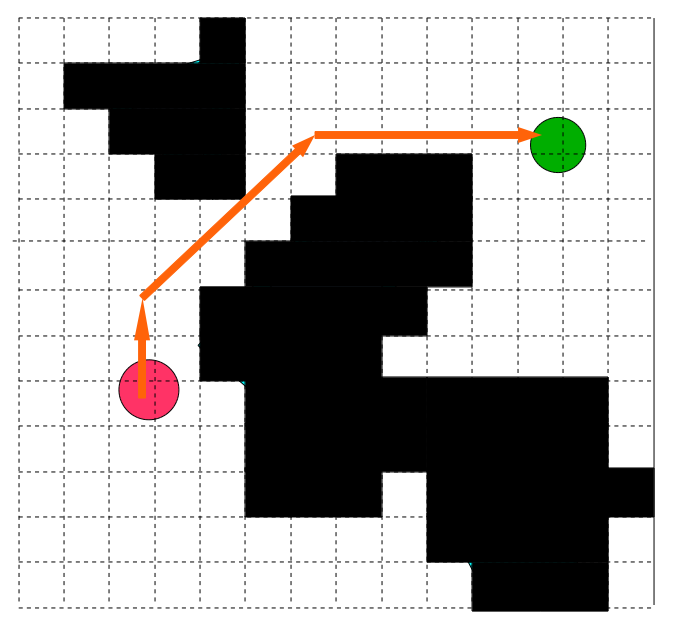
\includegraphics[width=0.3\textwidth,trim={0cm 0cm 0cm 0cm},clip]{exp_2d.png}
                    \end{center}
                    \begin{block}{Simulated: 2D}
                        \begin{itemize}
                            \item Simple 2D kinematics.
                            \item Applicable to numerous robots.
                            \item solutions may be unrealistic.
                        \end{itemize}
                    \end{block}
                    \begin{center}
                    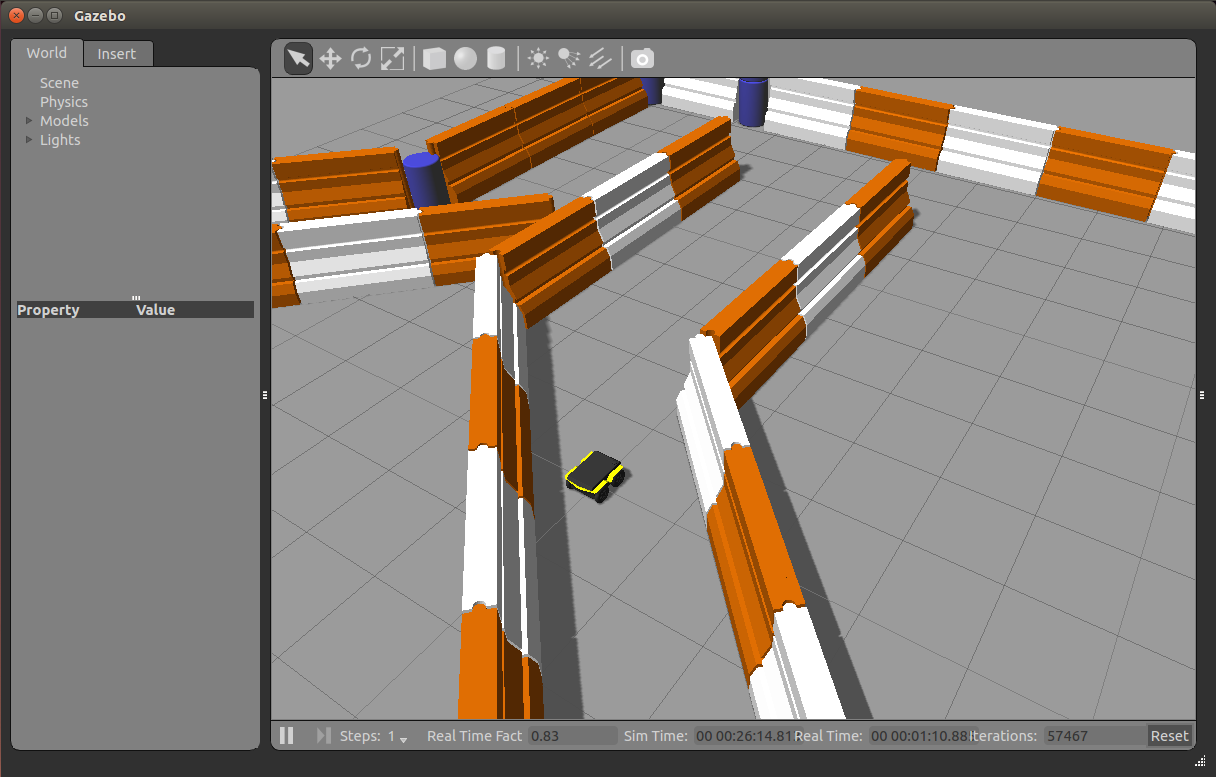
\includegraphics[width=0.4\textwidth,trim={0cm 0cm 0cm 0cm},clip]{exp_3d.png}
                    \end{center}
                    \begin{block}{Simulated: 3D}
                        \begin{itemize}
                            \item Closer to real life, model dynamics.
                        \end{itemize}
                    \end{block}                    
                \end{column}
                \begin{column}{0.5\textwidth}
                    \begin{center}
                    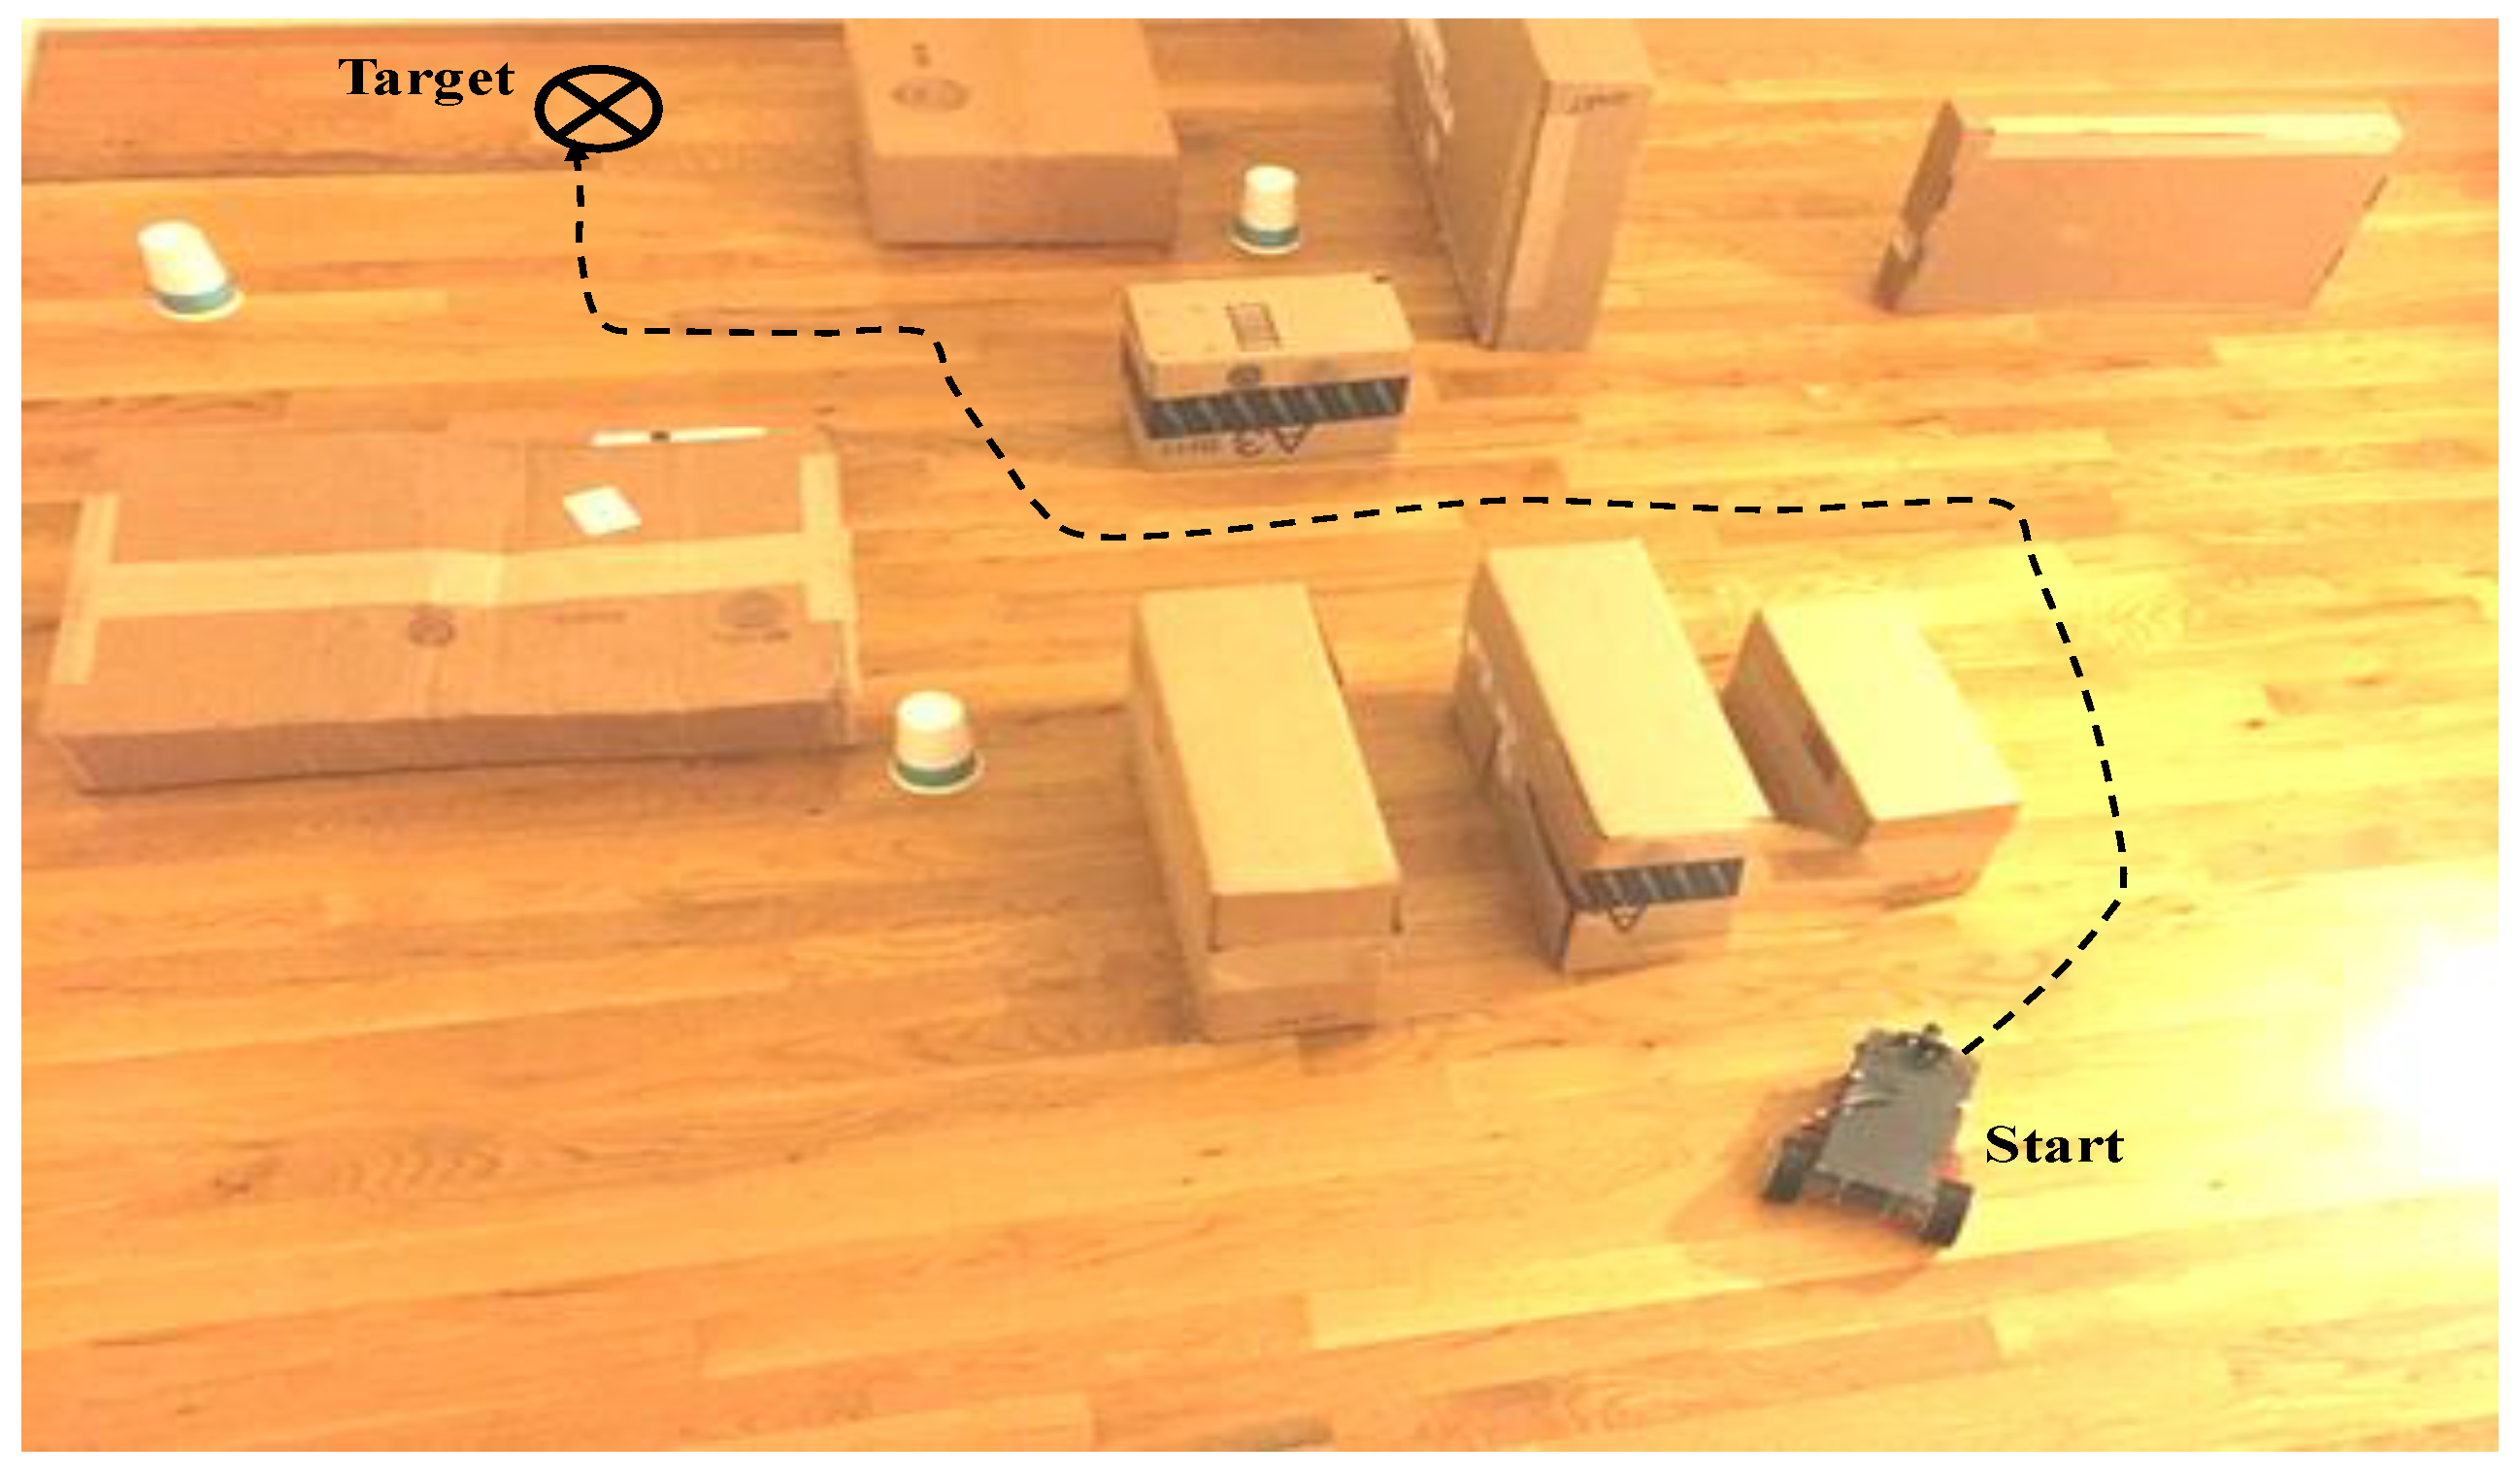
\includegraphics[width=0.8\textwidth,trim={0cm 0cm 0cm 0cm},clip]{exp_real.png}
                    \end{center}
                    \begin{block}{Real}
                        \begin{itemize}
                            \item Most realistic.
                            \item Very time-consuming.
                            \item May require engineering skills.
                            \item Forced to address real-world limitations.
                            \item Most impressive when completed. 
                        \end{itemize}
                    \end{block}
                \end{column}                
            \end{columns}           
        \end{block}
    \end{frame}
\end{section}

\begin{section}{Gazebo}
    \begin{frame}{Gazebo}
        Gazebo is 3D physics-based simulator for robotics.
        \begin{block}{Main Gazebo Features}
            \begin{itemize}
                \item \textbf{3D graphics.} \\
                Includes lighting, shadows, texture, etc.
                \item \textbf{Dynamic physics simulation.} \\
                Multiple physics engine available.
                \item \textbf{Various simulated, noisy sensors.} \\
                laser range finders, monocular \& stereo cameras, Kinect, etc. 
                \item \textbf{Numerous 3D robots.} \\
                Robots are models + physical characteristics. \\
                Several popular real robots have pre-made simulation counterparts. \\
                While tricky, possible to create own custom robots.
                \item \textbf{Plugin API} \\
                Can develop plugins that programatically affecting robots, sensors, or the environment. 
                \item Numerous existing plugins provide extensive ROS support. 
            \end{itemize}
        \end{block}
    \end{frame}
    \begin{frame}{Gazebo}
        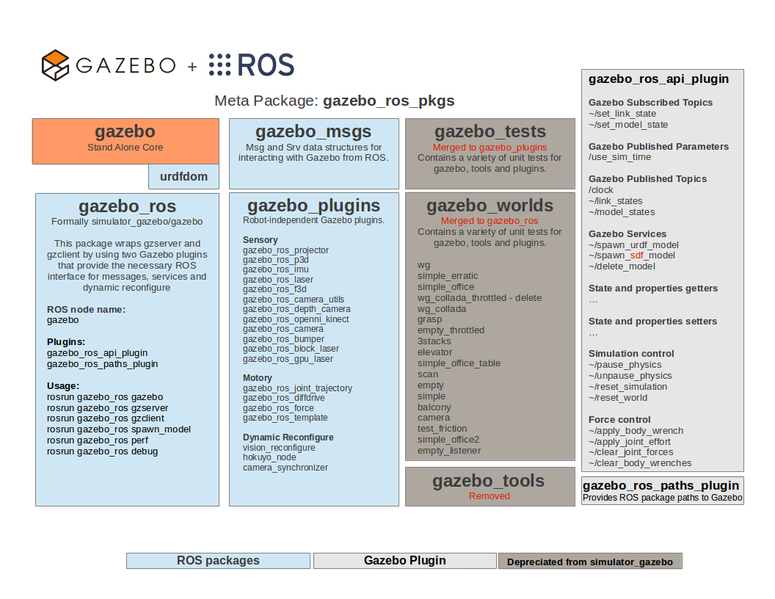
\includegraphics[width=\textwidth,trim={0cm 0cm 0cm 0cm},clip]{gazebo_overview.png}    
    \end{frame}
    \begin{frame}{Gazebo}
        \begin{block}{Example pipeline using OpenRAVE motion planner}
            \centering
            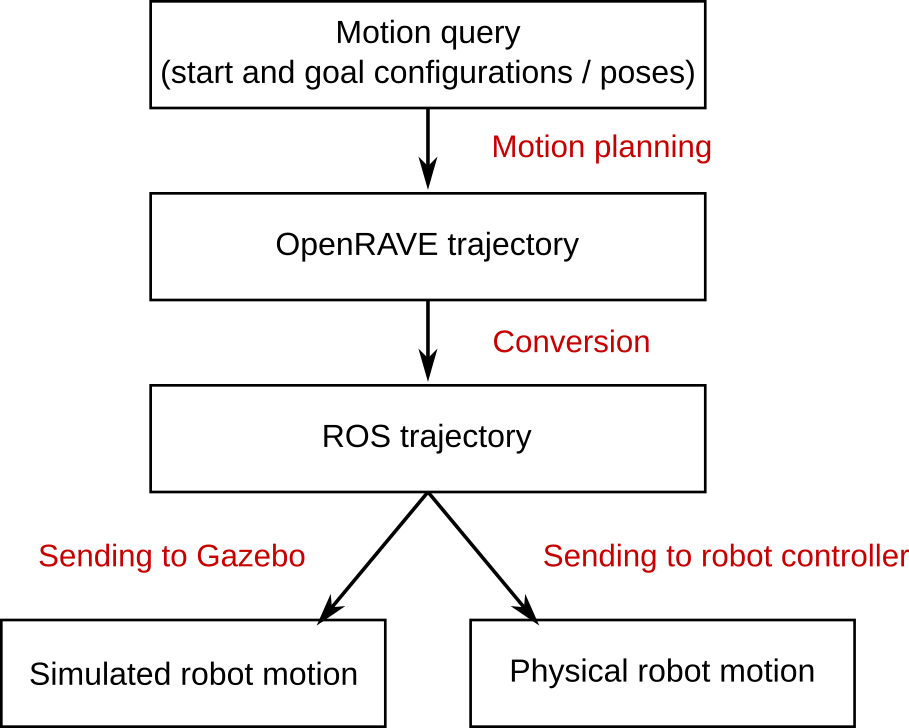
\includegraphics[width=0.8\textwidth,trim={0cm 0cm 0cm 0cm},clip]{robot_simulation_pipeline.png}
        \end{block}
    \end{frame}    
    
    \begin{frame}{Gazebo}
        \begin{block}{Getting Started Resources}
            \begin{itemize}
                \item [VIDEO] \textbf{Gazebo quick start, with Turtlebot}: \\
                \url{www.youtube.com/watch?v=9U6GDonGFHw}
                \item [VIDEO] \textbf{Robots and sensors from scratch}: \\
                \url{www.youtube.com/watch?v=8ckSl4MbZLg}
                \item Basic tutorials (Turtlebot): \\
                \url{learn.turtlebot.com/2015/02/03/3/}
                \item \textbf{Gazebo tutorials}: \\
                \url{github.com/SMARTlab-Purdue/ros-tutorial-gazebo-simulation}
                \item \textbf{Use \textit{Fetch} and \textit{Freight} robots}: \\
                \url{docs.fetchrobotics.com/gazebo.html}
                \item \textbf{Modify Gazebo environment through ROS topics}: \\
                \url{gazebosim.org/tutorials/?tut=ros_comm}
                \item \textbf{Gazebo + ROS + MATLAB}: \\
                \url{mathworks.com/help/robotics/examples/get-started-with-gazebo-and-a-simulated-turtlebot.html} \\
                Their examples avoid plugins by working with ROS topics. 
                Includes prebuilt virtual machine with Turtlebot for easy learning.
            \end{itemize}
        \end{block}
    \end{frame}
    \begin{frame}{Gazebo}
        \begin{block}{Challenges}
        Gazebo offers a wealth of resources. Many projects can be done by combining existing tools without too much trouble. However, custom functionality requires a rather steep learning curve.
            \begin{itemize}
                \item Documentation is extensive, but non-trivial to navigate. 
                \item Many significant plugins have minimal comments. \\
                \item Examples for using existing plugins might be sparse. 
                \item Seemingly routine tasks requires writing plugins in Gazebo's verbose, complex API. 
                \item Compiling plugins typically requires working with ROS's intricate catkin build system. 
                \item Some confusion exists between Gazebo topics and ROS topics, with overlap. \\
                Gazebo can exist outside of ROS, so it has own commands for pub/sub to topics. \\
                But plugins might be running that pushes some or all of the Gazebo topics to ROS topics. 
            \end{itemize}
        \end{block}
    \end{frame}
    
\end{section}    
    
\begin{section}{Examples}
    \begin{frame}{Example}
    \begin{columns}
        \begin{column}{0.5\textwidth}
            \begin{block}{Rover}
                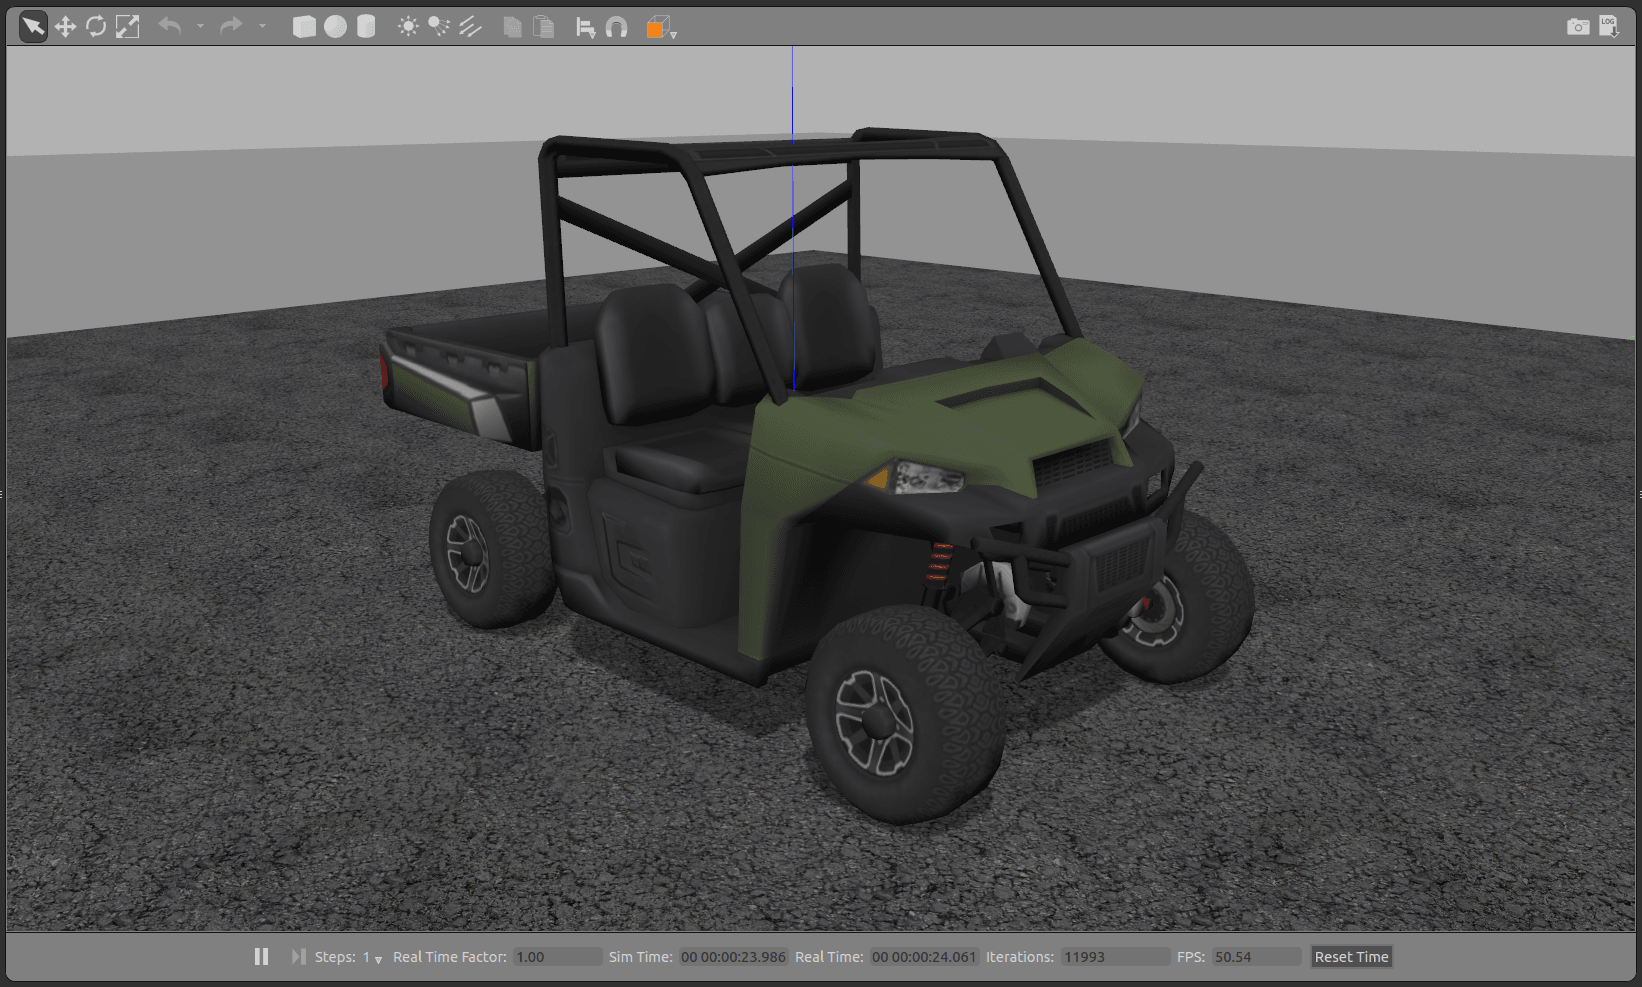
\includegraphics[width=0.8\textwidth,trim={0cm 0cm 0cm 0cm},clip]{rover.png}
            \end{block}
            \begin{block}{Quadcopter}        
                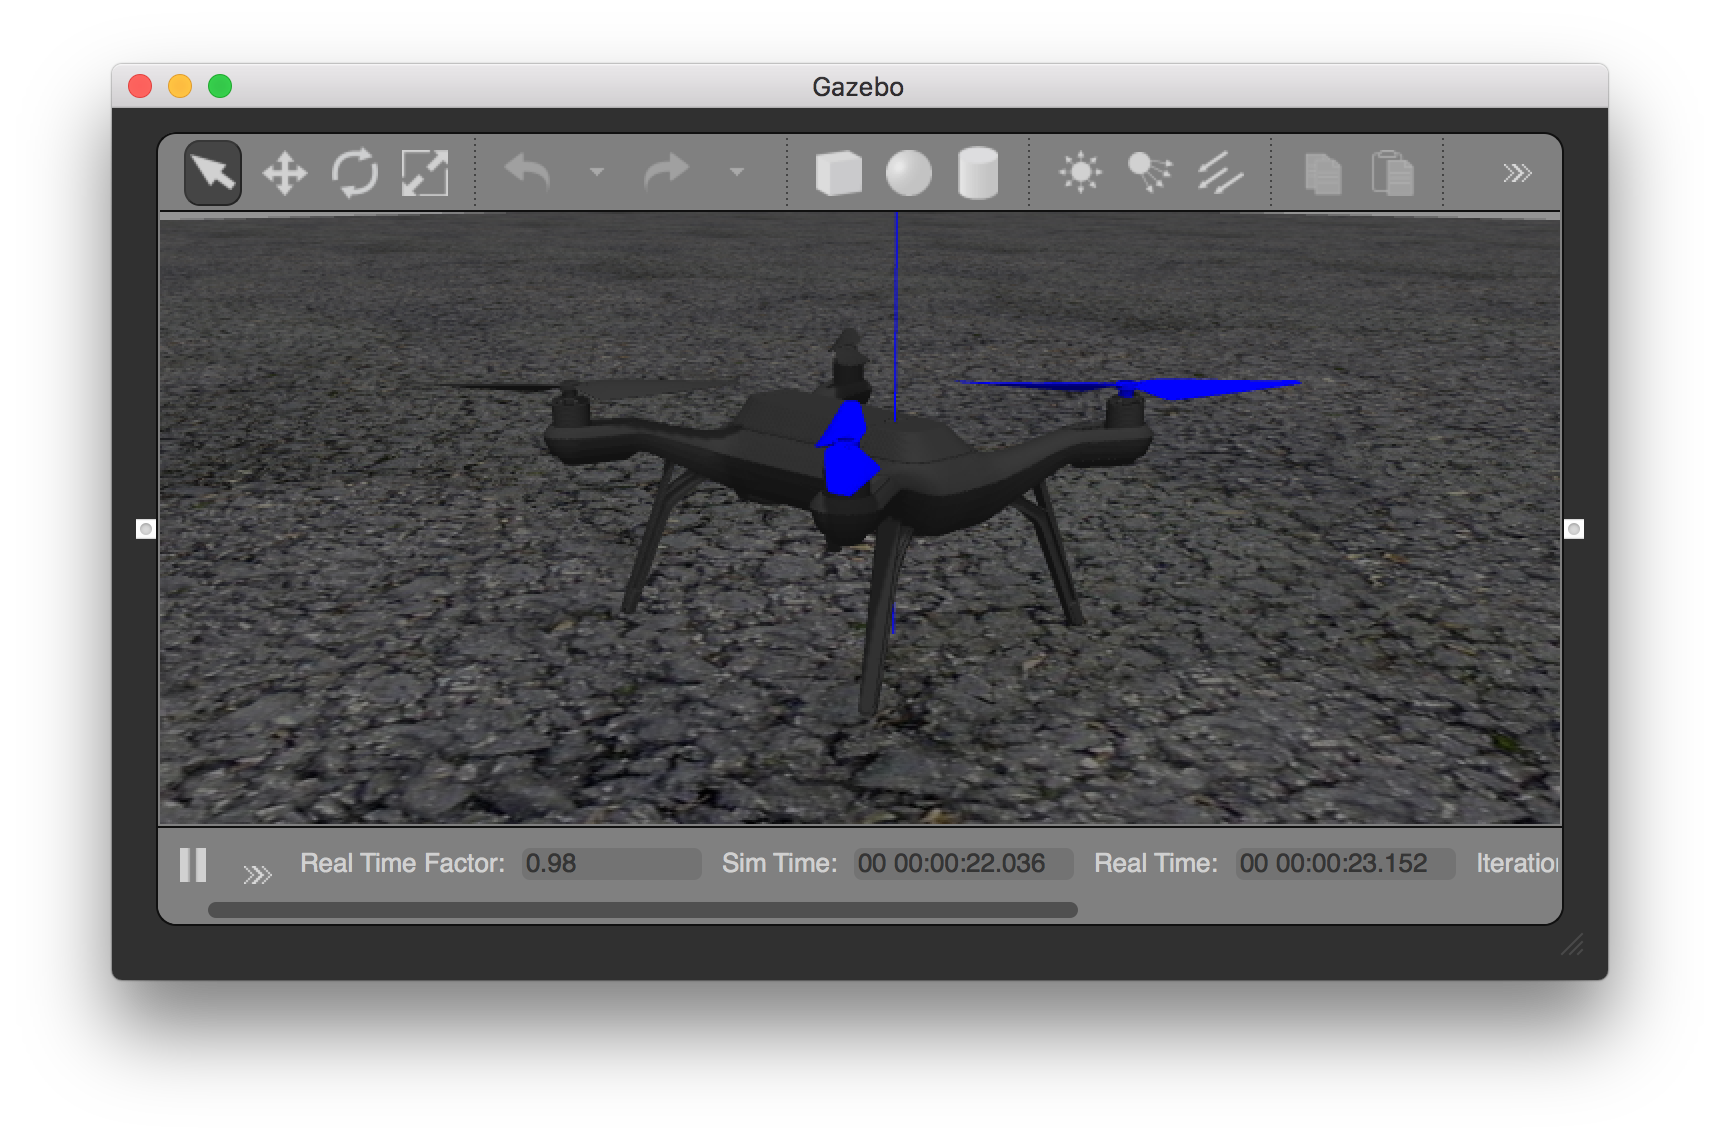
\includegraphics[width=0.9\textwidth,trim={0cm 0cm 0cm 0cm},clip]{solo.png}
            \end{block}
        \end{column}
        \begin{column}{0.5\textwidth}
            \begin{block}{UAV}            
                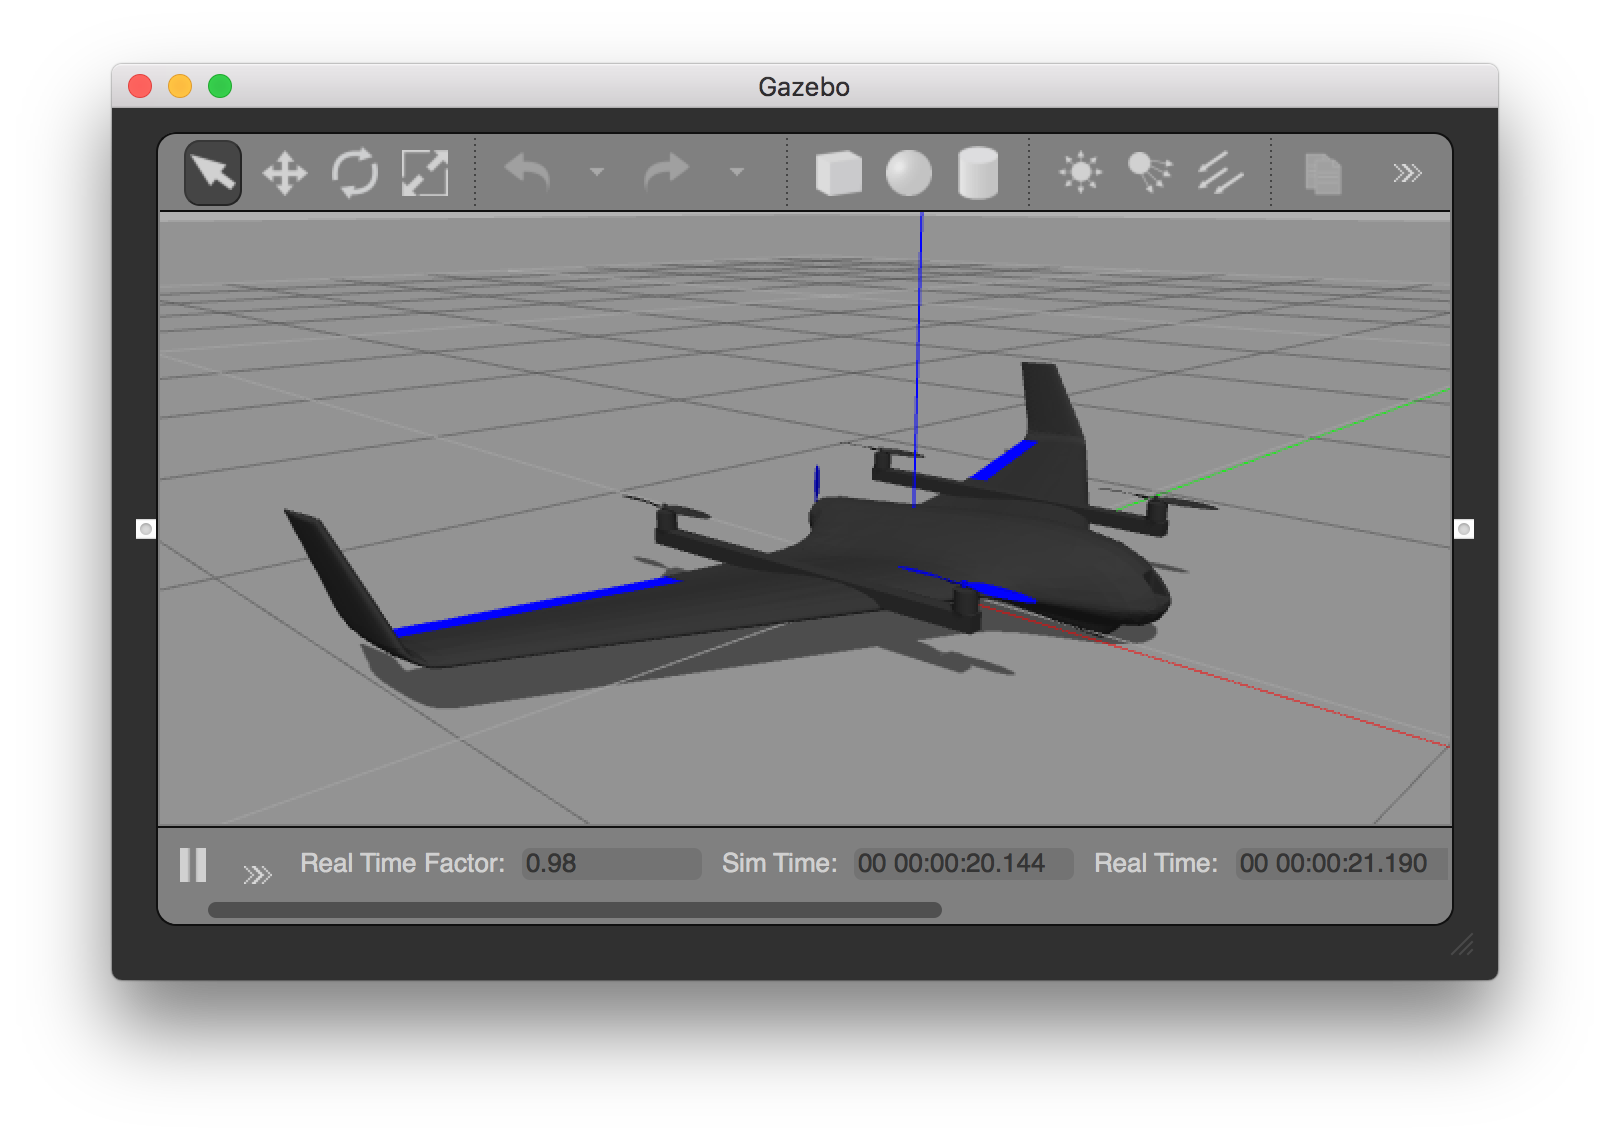
\includegraphics[width=0.9\textwidth,trim={0cm 0cm 0cm 0cm},clip]{standard_vtol.png}
            \end{block}
            \begin{block}{Unmanned Underwater Vehicle}            
                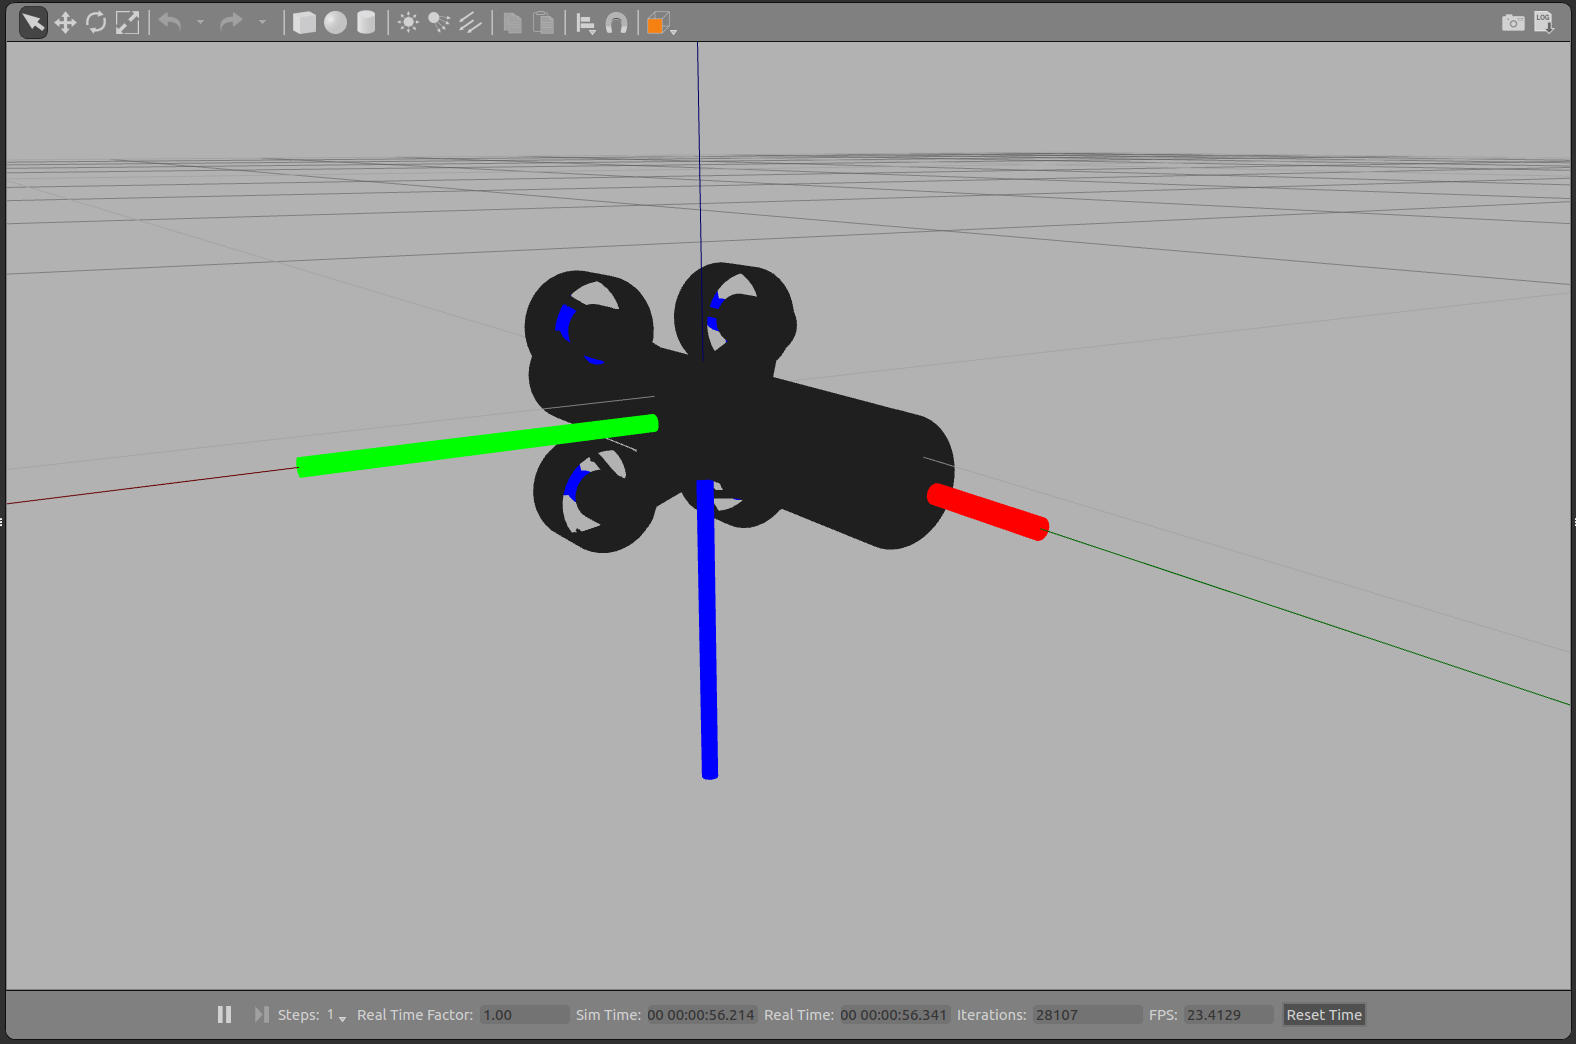
\includegraphics[width=0.8\textwidth,trim={0cm 0cm 0cm 0cm},clip]{hippocampus.png}
            \end{block}
        \end{column}        
    \end{columns}
    \end{frame}
    
    \begin{frame}{Example}
        \begin{block}{Laser Scanner}
            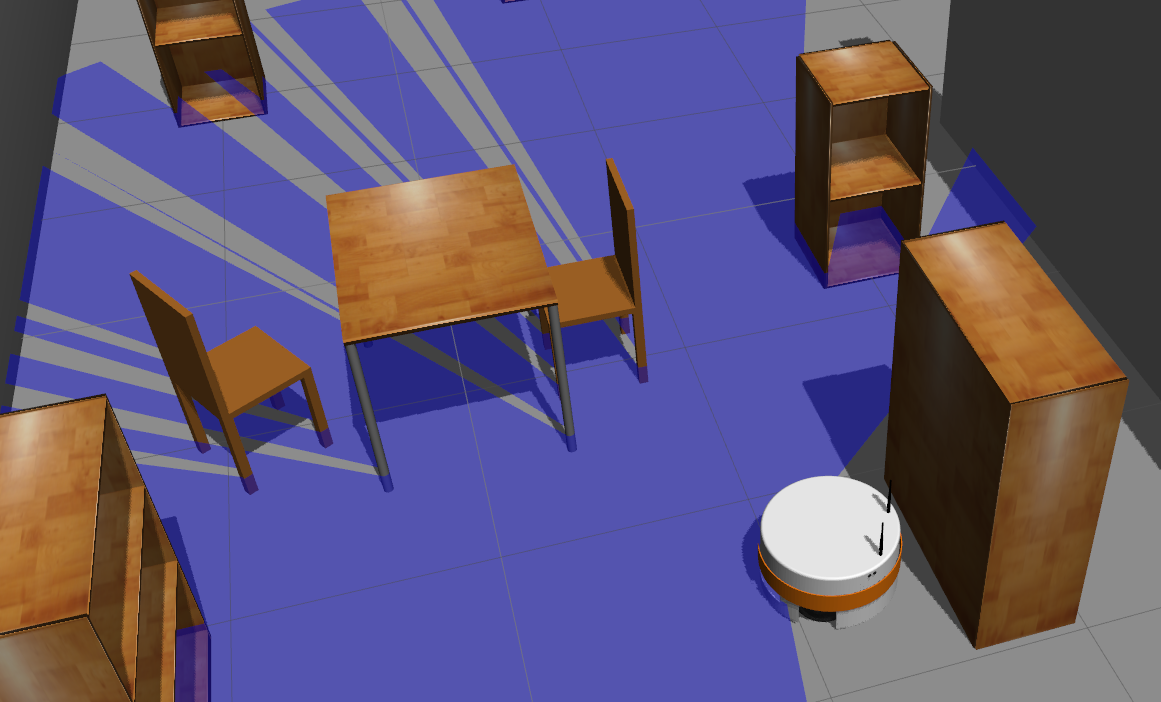
\includegraphics[width=\textwidth,trim={0cm 0cm 0cm 0cm},clip]{laserscanner.png}
        \end{block}
    \end{frame}

    \begin{frame}{Example}
        \begin{block}{3D Map Generation}
            \begin{columns}
                \begin{column}{0.5\textwidth}
                    \begin{block}{Two Robot Team}
                        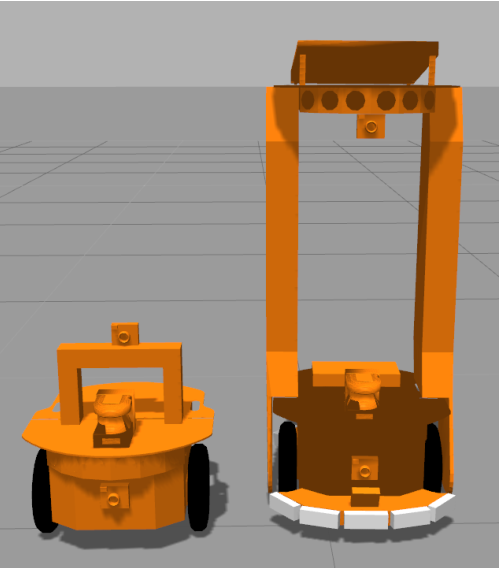
\includegraphics[width=0.8\textwidth,trim={0cm 0cm 0cm 0cm},clip]{3-Figure2-1.png}
                    \end{block}
                \end{column}
                \begin{column}{0.5\textwidth}
                    \begin{block}{Gazebo Environment}
                        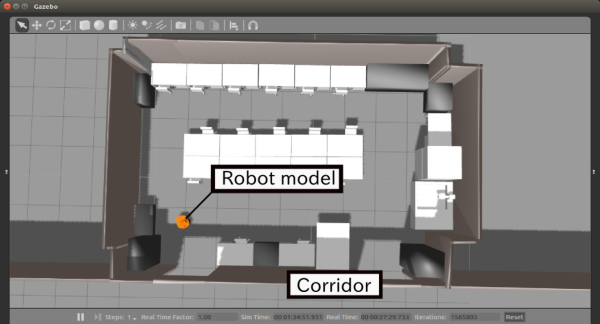
\includegraphics[width=0.9\textwidth,trim={0cm 0cm 0cm 0cm},clip]{3-Figure3-1.png}
                    \end{block}
                    \begin{block}{Mapping Visualization}
                        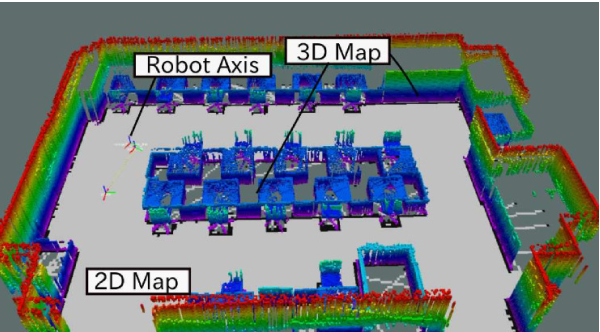
\includegraphics[width=0.9\textwidth,trim={0cm 0cm 0cm 0cm},clip]{5-Figure8-1.png}
                    \end{block}                    
                \end{column}
            \end{columns}
        \end{block}
    \end{frame}
    
    \begin{frame}{Example}
        \begin{block}{Path Planning using Particle Swarm Optimization}
            {\small 
            \textit{Collision-Free Autonomous Robot Navigation System Utilizing PSO for Path Planning in Unknown Environment} \\
            Evan Krell, Alaa Sheta, Arun Prassanth Ramaswamy Balasubramanian, Scott A. King \\
            Accepted in \textit{Journal of Artificial Intelligence and Soft Computing Research} (JAISCR) \\
            \url{https://github.com/ekrell/RobotPathPlanningPSO} \\
            }
            \centering
            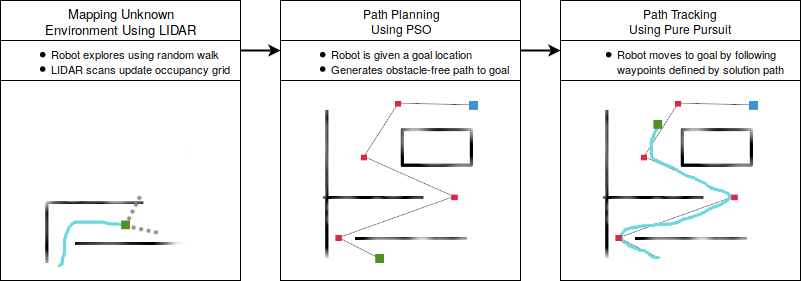
\includegraphics[width=0.8\textwidth,trim={0cm 7cm 0cm 0cm},clip]{sysoverview(1).png}
            \begin{columns}
                \begin{column}{0.5\textwidth}
                    \centering
                    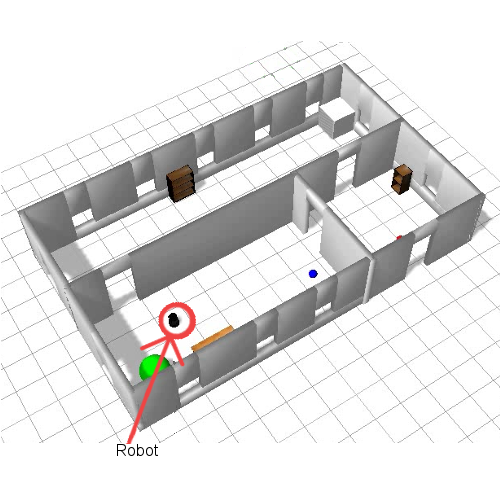
\includegraphics[width=0.7\textwidth,trim={0cm 0cm 0cm 0cm},clip]{Setup1.png}
                \end{column}
                \begin{column}{0.5\textwidth}
                    \centering
                    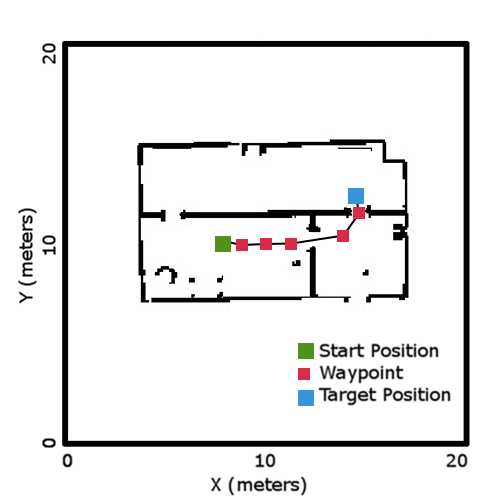
\includegraphics[width=0.7\textwidth,trim={0cm 0cm 0cm 0cm},clip]{PSO_Setup1_Run1.png}
                \end{column}            
            \end{columns}
        \end{block}
    \end{frame}
\end{section}

\begin{section}{Tutorials}
    \begin{frame}{Tutorial}
        \begin{block}{Tutorial: Create Robot and Sensor}
            \begin{itemize}
                \item We will watch the video tutorial, but pausing to analyze the code. 
                \item Video: \url{www.youtube.com/watch?v=8ckSl4MbZLg}
                \item Code: \url{github.com/richardw05/mybot_ws}
            \end{itemize}
        \end{block}
    \end{frame}
\end{section}

\begin{section}{Multirotor Simulation with RotorS}
    \begin{frame}{Multirotor Simulation with RotorS}
    \begin{columns}
        \begin{column}{0.5\textwidth}
            \centering
            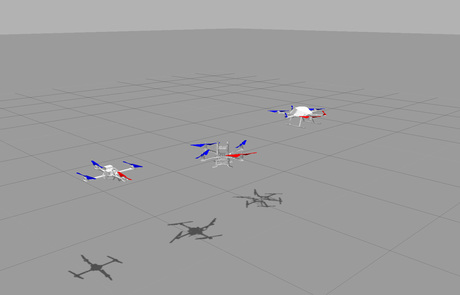
\includegraphics[width=0.7\textwidth,trim={0cm 0cm 0cm 0cm},clip]{rotors.jpg} \\
            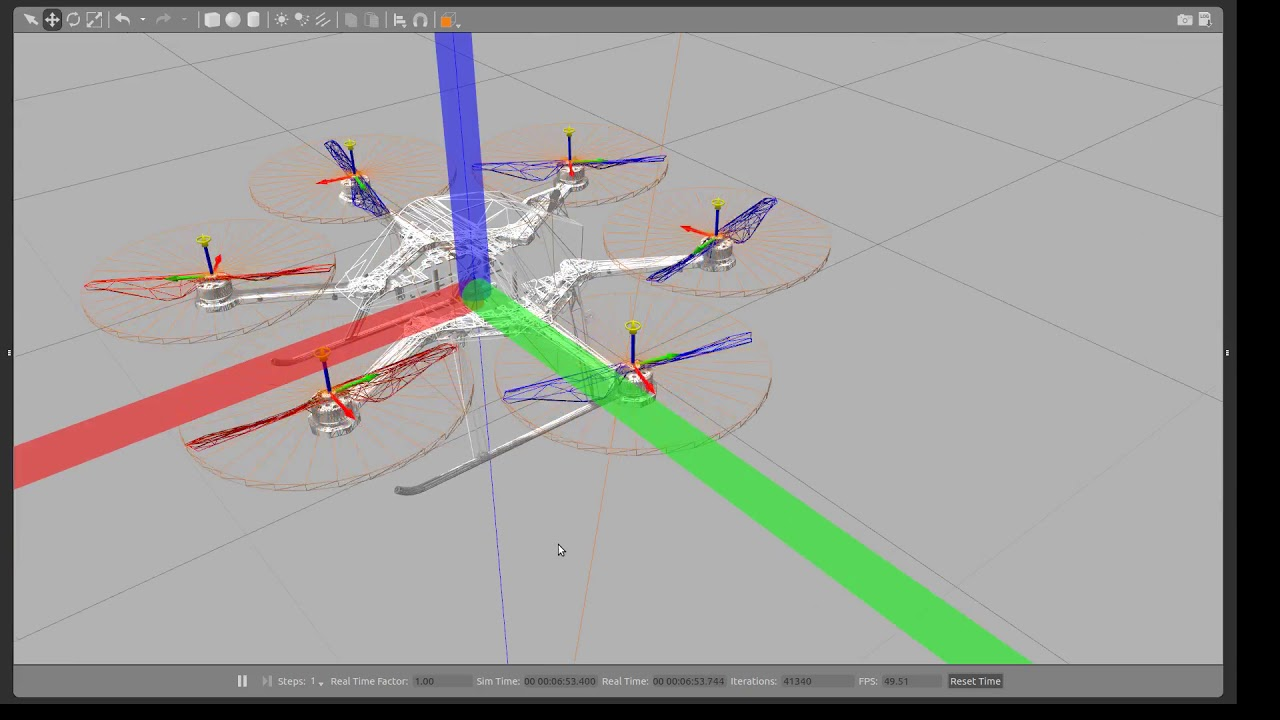
\includegraphics[width=0.7\textwidth,trim={0cm 0cm 0cm 0cm},clip]{rotors_zoom.jpg} \\ 
        \url{www.kostasalexis.com/rotors-simulator1.html}
        \end{column}
        \begin{column}{0.5\textwidth}
            \begin{block}{RotorS}
                \begin{itemize}
                    \item Multirotor simulation
                    \item Three \textit{AscTec} vehicles: Hummingbird, Pelican, Firefly.
                    \item Can add custom aircraft. 
                    \item Equipped with sensors: IMU, odometry, and Visual-Inertial (VI-) Sensor.
                    \item Includes waypoint-following (autopilot) and hovering packages. 
                    \item Can build and test custom controllers. 
                    \item Comes with a joystick interface. 
                    \item Minimal tutorials \& less documented than Turtlebot and other beginner-friendly packages. 
                \end{itemize}
            \end{block}
        \end{column}            
    \end{columns}
    \end{frame}
\end{section}

\begin{section}{Image Sources}
\begin{frame}{Image Sources}
\url{osrobotics.org/osr/system/simulation.html}
\url{https://dev.px4.io/en/simulation/gazebo.html}
\url{http://blog.pal-robotics.com/ros-simulation-available-for-pmb-2-tiagos-mobile-base/}
\url{Takaya, Kenta et al. “Simulation environment for mobile robots testing using ROS and Gazebo.” 2016 20th International Conference on System Theory, Control and Computing (ICSTCC) (2016): 96-101.}
\url{https://github.com/ethz-asl/rotors_simulator}
\end{frame}
\end{section}

\end{document}